% !TEX root = ./Vorlesungsmitschrift AGLA 2.tex  
\file{Desargues Pappos}
\subsection*{Zwei Anwendungen des Doppelverhältnisses}
\begin{satz}[Desargues]
  Sei \( \projectionspace{V} \) eine projektive Ebene und
  \begin{equation*}
    p_1,p_2,p_3,p_1',p_2',p_3' 
  \end{equation*}
  paarweise verschieden, sodass die Geraden
  \begin{equation*}
    p_1\vee p_1',p_2\vee p_2',p_3\vee p_3'
  \end{equation*}
  sich paarweise in einem gemeinsamen Punkt \( z \) schneiden.

  Dann sind die Schnittpunkte
  \begin{align*}
    a&\definedas (p_1\vee p_2)\cap (p_1'\vee p_2')\\
    b&\definedas (p_2\vee p_3)\cap (p_2'\vee p_3')\\
    c&\definedas (p_3\vee p_1)\cap (p_3'\vee p_1')
  \end{align*}
  in einer Geraden enthalten.
\end{satz}
\begin{proof}
  \begin{figure}
    \centering
    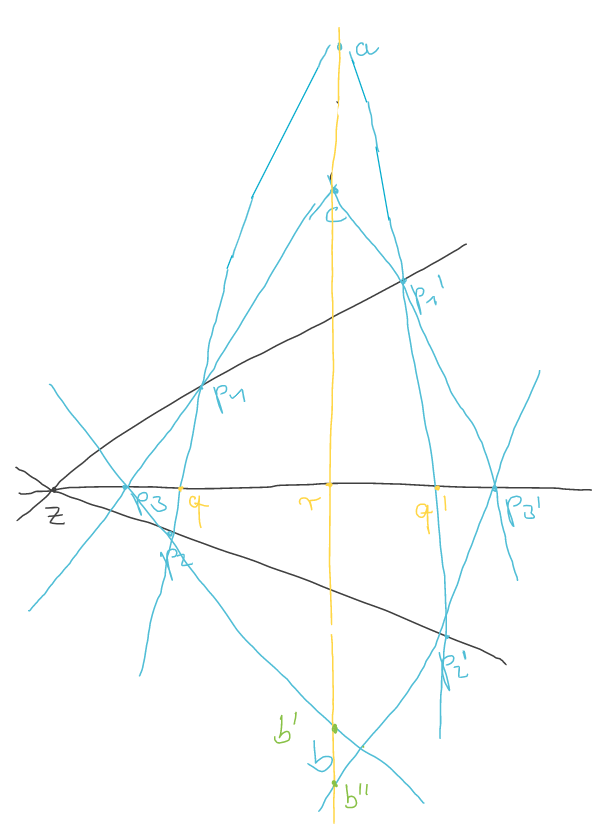
\includegraphics[width=0.9\linewidth]{desargues_visualisierung}
    \label{fig:desargues_visualisierung}
  \end{figure}
  Sei
  \begin{align*}
    q&\definedas (p_1\vee p_2)\cap (p_3\vee p_3')\\
    q'&\definedas (p_1\vee p_2')\cap (p_3\vee p_3')\\
    r&\definedas (a\vee c)\cap (p_3\vee p_3')\\
    b'&\definedas (a\vee c) \cap (p_2\vee p_3)\\
    b''&\definedas (a\vee c)\cap (p_2'\vee p_3')
  \end{align*}
  
  \begin{ziel*}
    Wir zeigen \( b'=b'' \), denn dann ist
    \begin{equation*}
      b'\cap b''\in (a\vee c)\cap \braceannotate{b}{(p_2\vee p_3)\cap (p_2'\vee p_3')}.
    \end{equation*}
  \end{ziel*}
  Die Punkte \( a\), \( c \) und \( r \), sind paarweise verschieden, es genügt also zu zeigen, dass
  \begin{equation*}
    \doppelverhaeltnis{a}{c}{r}{b'}=\doppelverhaeltnis{a}{c}{r}{b''}.
  \end{equation*}
  Betrachte die Zentralprojektion
  \begin{equation*}
    f_1\maps a\vee c\to a\vee p_1
  \end{equation*}
  mit Zentrum \( p_3 \). Es folgt 
  \begin{equation*}
    \doppelverhaeltnis{a}{c}{r}{b'}=\doppelverhaeltnis{a}{p_1}{q}{p_2}.
  \end{equation*}
  Verwende als Nächstes die Zentralprojektion
  \begin{equation*}
    f_2\maps a\vee p_1\to  a\vee p_1'
  \end{equation*}
  mit Zentrum \( z \) und erhalte
  \begin{equation*}
    \doppelverhaeltnis{a}{p_1}{q}{p_2}=\doppelverhaeltnis{a}{p_1'}{q'}{p_2'}
  \end{equation*}
  und danach die Zentralprojektion
  \begin{equation*}
    f_3\maps a\vee p_1'\to a\vee c
  \end{equation*}
  mit Zentrum \( p_3' \). Dann ist
  \begin{equation*}
    \doppelverhaeltnis{a}{p_1'}{q'}{p_2'}=\doppelverhaeltnis{a}{c}{r}{b''},
  \end{equation*}
  also
  \begin{equation*}
    \doppelverhaeltnis{a}{c}{r}{b'}=\doppelverhaeltnis{a}{c}{r}{b''}.
  \end{equation*}
\end{proof}
\begin{satz}[Pappos]
  Seien \( z,z'\subset \projectionspace{V} \) verschiedene Geraden in einer projektiven Ebene und
  \begin{equation*}
    p_1,p_2,p_3,p_1',p_2',p_3'
  \end{equation*}
  paarweise verschiedene Punkte mit
  \begin{align*}
    p_1,p_2,p_3&\in Z\\
    p_1',p_2',p_3'&\in Z'.
  \end{align*}
  Dann sind die Punkte
  \begin{align*}
    a&\definedas (p_1\vee p_2')\cap (p_1'\vee p_2)\\
    b&\definedas (p_2\vee p_3')\cap (p_2'\vee p_3)\\
    c&\definedas (p_3\vee p_1')\cap (p_3'\vee p_1)
  \end{align*}
  in einer Geraden enthalten.
\end{satz}
\begin{proof}
  \begin{figure}
    \centering
    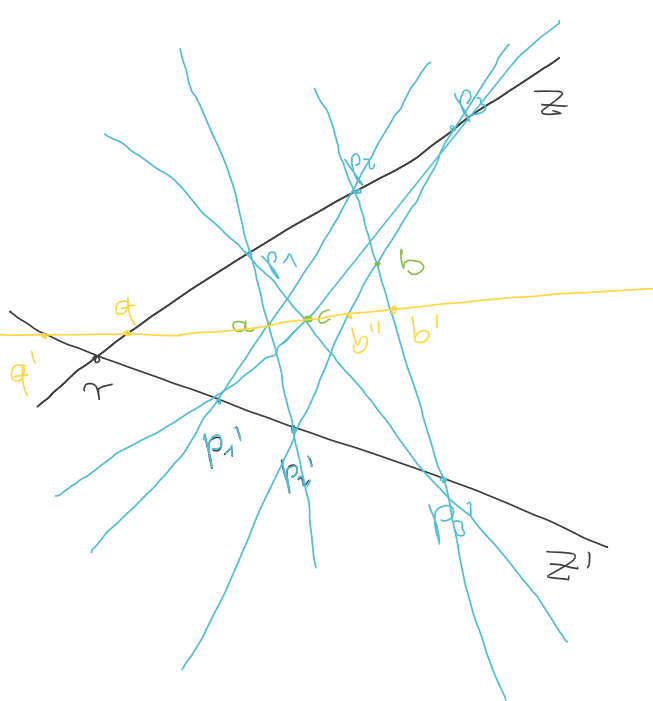
\includegraphics[width=\linewidth]{pappos_visualisierung}
    \label{fig:pappos_visualisierung}
  \end{figure}
  Wir definieren
  \begin{align*}
    r&\definedas Z\cap Z'\\
    q&\definedas (a\vee c)\cap Z\\
    q'&\definedas (a\vee c)\cap Z'\\
    b'&\definedas (a\vee c)\cap (p_2\vee p_3')\\
    b''&\definedas (a\vee c)\cap(p_2'\vee p_3).
  \end{align*}
  Falls 
  \begin{equation*}
    r\in \set{p_1,p_2,p_3,p_1',p_2',p_3'},
  \end{equation*}
  \zb \( r=p_1 \), dann sind \( a,b,c \) in der Geraden \( p_1'\vee b \) enthalten. Ebenso können wir 
  \begin{equation*}
    a\in \set{p_1,p_2,p_3,p_1',p_2',p_3'}
  \end{equation*}
  Wir nehmen also an
  \begin{equation*}
    a,r\not\in \set{p_1,p_2,p_3,p_1',p_2',p_3'}.
  \end{equation*}
  \begin{ziel*}
    Zeige, dass \( b'=b'' \).
  \end{ziel*}
  Wir verwenden Zentralprojektionen
  \begin{equation*}
    f_1\maps a\vee c\to \braceannotate{Z}{p_1\vee p_2}
  \end{equation*}
  mit Zentrum \( p_3' \),
  \begin{equation*}
    \doppelverhaeltnis{q}{c}{q'}{b'}=\doppelverhaeltnis{q}{p_1}{r}{p_2}.
  \end{equation*}
  Danach
  \begin{equation*}
    f_2\maps \braceannotate{Z}{p_1\vee p_2}\to Z'
  \end{equation*}
  mit Zentrum \( a \),
  \begin{equation*}
    \doppelverhaeltnis{q}{p_1}{r}{p_2}=\doppelverhaeltnis{q'}{p_2'}{r}{p_1'}.
  \end{equation*}
  Verwende dann die Zentralprojektion
  \begin{equation*}
    f_3\maps Z'\to a\vee c
  \end{equation*}
  mit Zentrum \( p_3 \),
  \begin{equation*}
    \doppelverhaeltnis{q'}{p_2'}{r}{p_1'}=\doppelverhaeltnis{q'}{b''}{q}{c}.
  \end{equation*}
  Nach Symmetrie gilt
  \begin{equation*}
    \doppelverhaeltnis{q'}{b''}{q}{c}=\doppelverhaeltnis{q}{c}{q'}{b''}
  \end{equation*}
  und damit \( b'=b'' \).
\end{proof}
\file{Hauptsatz projektive Geometrie}
\section{Hauptsatz der projektiven Geometrie}
Seien \( V,W \) \( K \)-Vektorräume und
\begin{equation*}
  f\maps \projectionspace{V}\to\projectionspace{W}
\end{equation*}
eine Projektivität. Ist \( Z\subseteq \projectionspace{V} \) eine projektive Gerade, so ist auch
\begin{equation*}
  f(Z)\subseteq \projectionspace{W}
\end{equation*}
eine projektive Gerade.

\begin{frage*}
  Welche bijektiven Abbildungen
  \begin{equation*}
    g\maps \projectionspace{V}\to \projectionspace{W}
  \end{equation*}
  haben die Eigenschaft, dass Geraden auf Geraden abgebildet werden?
\end{frage*}
\begin{definition*}
  Seien \( V,W \) \( K \)-Vektorräume und \( g\maps \projectionspace{V}\to \projectionspace{W} \) eine bijektive Abbildung, sodass \( \forall p,p'\in \projectionspace{V} \)
  \begin{equation*}
    f(p\vee p')\subseteq f(p)\vee f(p').
  \end{equation*}
  Dann nennen wir \( g \) Kollineation.
\end{definition*}
\begin{beispiel*}
  Sei \( K \) ein Körper mit Automorphismus \( \alpha \) und \( F\maps V\to W \) eine injektive   lineare Abbildung, \dh 
  \begin{align*}
    F(v+v')&=F(v)+F(v')\quad \forall v,v'\in V\\
    F(\lambda v)&=\alpha(\lambda)F(v)\quad \forall \lambda\in K\logicspace \forall v\in V.
  \end{align*}
  Dann induziert \( F \) eine Abbildung
  \begin{equation*}
    \begin{split}
      \projectionmap{F}\maps \projectionspace{V}\%to \projectionspace{W}\\
      \projectionspace{V}\ni K\cdot v&\mapsto K\cdot F(v)\quad v\in V\setminus\zeroset.
    \end{split}
  \end{equation*}
\end{beispiel*}

\begin{definition*}
  Seien \( V,W \) \( K \)-Vektorräume. Wir nennen eine Abbildung
  \begin{equation*}
    f\maps \projectionspace{V}\to \projectionspace{W}
  \end{equation*}
  \emph{semiprojektiv}, falls es eine injektive semilineare Abbildung \( F\maps V\to W \) gibt mit
  \begin{equation*}
    f=\projectionmap{F}.
  \end{equation*}
  Falls \( f \) außerdem bijektiv ist, so nennen wir \( f \) Semiprojektivität.
\end{definition*}
\begin{bemerkung*}
  Ist \( F\maps V\to W \) semilinear, so gilt
  \begin{equation*}
    F(K\cdot v)=K\cdot F(v),
  \end{equation*}
  dnn
  \begin{align*}
    F(K\cdot v)&=\Set{F(\lambda v)|\lambda\in K}\\
    &=\Set{\alpha(\lambda)F(v)|\lambda\in K}\\
    &\explain{\alpha \text{ ist bijekti}}{=}\Set{\lambda F(v)|\lambda\in K}\\
    &=K\cdot F(v).
  \end{align*}
\end{bemerkung*}
\begin{beispiel*}
  Betrachte den Körper
  \begin{equation*}
    \rationals(\sqrt{2})=\Set{a+b\sqrt{2}|a,b\in \rationals}
  \end{equation*}
  mit Automorphismus
  \begin{equation*}
    a+b\sqrt{2}\mapsto a-b\sqrt{2}\quad a,b\in \rationals.
  \end{equation*}
  Dann ist
  \begin{equation}
    \begin{split}
      F\maps \rationals(\sqrt{2})^3&\to \rationals(\sqrt{2})^3\\
      (a_1+b_1\sqrt{2},a_2+b_2\sqrt{2},a_3+b_3\sqrt{2})&\mapsto (a_1-b_1\sqrt{2}, a_2-b_2\sqrt{2},a_3-b_3\sqrt{2})
    \end{split}
  \end{equation}
  eine semilineare Abbildung, die eine Semiprojektivität
  \begin{equation*}
    \projectionmap{F}\maps \projectionspaceover{2}{\rationals(\sqrt{2})}\to\projectionspaceover{2}{\rationals(\sqrt{2})}
  \end{equation*}
  induziert.
\end{beispiel*}
\begin{frage*}
  Ist \( \projectionmap{F} \) eine Projektivität über \( \rationals(\sqrt{2}) \)?
\end{frage*}
\begin{lemma}
  Seien \( V,W \) \( K \)-Vektorräume, \( f\maps \projectionspace{V}\to \projectionspace{W} \) eine semiprojektive Abbildung und \( Z\subseteq \projectionspace{V} \) ein projektiver Unterraum. Dann ist \( f(Z)\subseteq \projectionspace{W} \) ein projektiver Unterraum mit 
  \begin{equation*}
    \projectivedim-{f(Z)}=\projectivedim-{Z}.
  \end{equation*}
\end{lemma}
\begin{proof}
  Sei \( Z=\projectionspace{U} \) mit \( U\untervektorraum V \) \( K \)-Untervektorraum,
  \begin{equation*}
    \dim-{}{U}=\projectivedim-{Z}+1=r.
  \end{equation*}
  Sei \( F\maps V\to W \) injektiv, semilinear zum Automorphismus \( \alpha \) und \( f=\projectionmap{F} \). Sei \( v_1,\dotsc,v_r\in V \) eine Basis von \( U \) als \( K \)-Vektorraum. Wir berechnen
  \begin{align*}
    F(U)&=F(K\cdot v_1+\dotsb+K v_r)\\
    &=\Set{F(\lambda_1 v_1+\dotsb+\lambda_r v_r)|\lambda_1,\dotsc,\lambda_r\in K}\\
    &\explain{F \text{ ist semilinear}}{=}\Set{\alpha(\lambda_1)F(v_1)+\dotsb+\alpha(\lambda_r)F(v_r)|\lambda_1,\dotsc,\lambda_r\in K}
    &=\Set{\lambda_1 F(v_1)+\dotsb+\lambda_r F(v_r)|\lambda_1,\dotsc,\lambda_r\in K}\\
    &=K\cdot F(v_1)+\dotsb+K\cdot F(v_r)
  \end{align*}
  ist \( K \)-Untervektorraum on \( W \). Es ist \( \dim-{}{F(U)}=r \), da \( F \) injektiv + semilinear ist. Verwende nun
  \begin{equation*}
    f(Z)=\projectionspace{F(U)}.
  \end{equation*}  
\end{proof}
\begin{satz}[Hauptsatz der projektiven Geometrie]\label{hauptsatz_projektive_geometrie}
  Seien \( V,W \) \( K \)-Vektorräume mit \( \dim-{}{V}=\dim-{}{W}\geq 3 \) und \( f\maps \projectionspace{V}\to\projectionspace{W} \) eine Kollineation. Dann ist \( f \) eine Semiprojektivität.
\end{satz}
\begin{bemerkung*}
  Im Fall \( K=\reals \) folgt sogar, dass \( f \) eine Projektivität ist, \dh für reelle projektive Räume der Dimension \( \geq 2 \) sind die Begriffe Kollineation und Projektivität gleichbedeutend.
\end{bemerkung*}
\lecture{Di 16.06.}{}
\begin{proof}[Beweis von \thref{hauptsatz_projektive_geometrie}]
  Im Folgenden sei \( K \) ein Körper, \( V,W \) \( K \)-Vektorräume mit \( \dim-{}{V}=\dim-{}{W}\geq 3 \) und \( f\maps \projectionspace{V}\to \projectionspace{W} \) eine Kollineation.
  \begin{lemma}\label{kollineation_erhaelt_verbindungsraum}
    Seien \( p_0,\dotsc,p_r\in \projectionspace{V} \). Dann ist
    \begin{equation*}
      f(p_0 \vee \dotsb\vee p_r)\subseteq f(p_0)\vee \dotsb\vee f(p_r).
    \end{equation*}
  \end{lemma}
  \begin{subproof}
    Induktion über \( r \).
    \begin{proofdescription}
      \item[\( r=0 \)] \( f(p_0)\subseteq f(p_0) \) \checkmark.
      \item[\( r\geq 1 \)] \( p\in (p_0\vee \dotsb\vee p_{r-1})\vee p_r \) mit \( p_i=K\cdot v_i \), \( v_i\in V \), \( 0\leq i\leq r \). 

      Dann ist
      \begin{equation*}
        p_0\vee \dotsb\vee p_{r-1}\vee p_r=\projectionspace{K\cdot v_0+\dotsb+K\cdot v_r}
      \end{equation*}
      und
      \begin{equation*}
        \exists p'\in p_0\vee \dotsb\vee p_{r_1}=\projectionspace{Kv_0+\dotsb+Kv_{r-1}}
      \end{equation*}
      mit \( p\in p'\vee p_r \). Dann gilt
      \begin{align*}
        f(p)&\explain{f \text{ ist Kollineation}}{\in}f(p')\vee (p_r)\\
        &\in f(p_0)\vee \dotsb\vee f(p_{r-1})\vee f(p_r).
      \end{align*}
    \end{proofdescription}
  \end{subproof}
  \begin{lemma}\label{kollineation_verhaelt_sich_gut_mit_basen}
    Sei \( \dim-{}{V}=\dim-{}{W}=n+1 \). Dann gibt es Basen \( v_0,\dotsc,v_n \) von \( V \) und \( w_0,\dotsc,w_n \) von \( W \) mit der Eigenschaft
    \begin{equation*}
      f(K\cdot v_i)=K\cdot w_i\quad 0\leq i\leq n 
    \end{equation*}
    und 
    \begin{equation*}
      f(K\cdot (v_0+v_i))=K\cdot (w_0+w_i)1\leq i\leq n.
    \end{equation*}
  \end{lemma}
  \begin{subproof}
    Wähl eine Basis \( v_0,\dotsc,v_n \) von \( V \) und \( w_0',\dotsc,w_n'\in W \), sodass
    \begin{equation*}
      f(K\cdot v_i)=K\cdot w_i'\quad 0\leq i\leq n.
    \end{equation*}
    Es ist
    \begin{align*}
      \projectionspace{W}&=f(\projectionspace{V})\\
      &=f(K\cdot v_0\vee \dotsb\vee K\cdot v_n)\\
      &\explain{\text{\thref{kollineation_erhaelt_verbindungsraum}}}{\subseteq} f(K\cdot v_0)\vee \dotsb\vee f(K\cdot v_n)\\
      &=\projectionspace{K\cdot w_0'+\dotsb+K\cdot w_n'},
    \end{align*}
    also ist \( w_0',\dotsc,w_n' \) eine Basis von \( W \). Es gilt
    \begin{equation*}
      K\cdot (v_0+v_i)\in K\cdot v_0\vee K\cdot v_i,
    \end{equation*}
    also, da \( f \) Kollineation,
    \begin{align*}
      f(K\cdot (v_0+v_i))&\in \braceannotate{K\cdot w_0'}{f(K\cdot v_0)}\vee \braceannotate{K\cdot w_i'}{f(K\cdot v_i)}\\
      &\in K\cdot w_0'\vee K\cdot w_i', 
    \end{align*}
    also \texists \( \lambda_i,\mu_i\in K \), \( 1\leq i \leq n \) mit
    \begin{align*}
      f(K(v_0+v_i))&=K(\mu_i w_0'+\lambda_i w_i')\\
      &=K(w_0'+\inverse{\mu_i}\lambda_i w_i').
    \end{align*}
    Außerdem ist \( \lambda_i,\mu_i\neq 0\quad \forall i \), denn aus \( \lambda_i=0 \), \( \mu_i\neq 0 \) folgt \zb
    \begin{equation*}
      f(K\cdot(v_0+v_i))=K\cdot w_0'=f(K\cdot v_0),
    \end{equation*}
    \contra \( f \) ist bijektiv.

    Also ist \( \lambda_i, \mu_i\in \fieldwithoutzero{K}\quad \forall 1\leq i\leq n \).

    Setze nun \( w_0\definedas w_0' \) und \( w_i=\braceannotate{\in \fieldwithoutzero{K}}{\lambda_i \inverse{\mu_i}}w_i' \), \( 1\leq i\leq n \).
    
  \end{subproof}
  Im Folgenden seien \( v_0,\dotsc,v_n\in V\) und \( w_0,\dotsc,w_n\in W \) wie in \thref{kollineation_verhaelt_sich_gut_mit_basen}, \dh \( v_0,\dotsc,v_n \) ist Basis von \( V \), \( w_0,\dotsc, w_n \) ist Basis von \( W \) mit
  \begin{align*}
    f(K\cdot v_i)&=K\cdot w_i\quad 0\leq i\leq n\\
    f(K\cdot (v_0+ v_i))=K(w_0+w_i)\quad 1\leq i\leq n.
  \end{align*}
  \begin{lemma}\label{kollineation_hat_zugehoerigen_vielleicht_automorphismus}
    Es gibt ein injektive Abbildung
    \begin{equation*}
      \alpha\maps K\to K
    \end{equation*}
    mit \( \alpha(0)=0 \), \( \alpha(1)=1 \), und
    \begin{equation*}
      f(K\cdot (v_0+\lambda v_i))=K\cdot (w_0+\alpha(\lambda)w_i)\quad 1\leq i\leq n\logicspace \forall \lambda\in K.
    \end{equation*}
  \end{lemma}
  \begin{proof}
    Sei \( 1\leq i\leq n \) fest, \( \lambda\in K \). Setze
    \begin{equation*}
      p=K(v_0+\lambda v_i).
    \end{equation*}
    Dann ist \( p\in K\cdot v_0\vee K\cdot v_i \), also \( f(p)\in K\cdot w_0\vee K\cdot w_i \). Aus \( p\neq K\cdot v_i \) folgt \( f(p)\neq K\cdot w_i \) und es gibt \( \alpha_i(\lambda)\in K \) mit 
    \begin{equation*}
      f(p)=K\cdot (w_0+\alpha_i(\lambda)w_i).
    \end{equation*}
    Definiere \( \alpha_i\maps K\to K \), \( \lambda\mapsto \alpha_i(\lambda) \), \( \alpha_i \) ist injektiv, denn für \( \lambda_1\neq \lambda_2 \) ist
    \begin{equation*}
      K\cdot (v_0+\lambda_1 v_i)\neq K\cdot (v_0\lambda_2 v_i).
    \end{equation*}
    Nach Konstruktion von \( v_0,\dotsc,v_n \), \( w_0,\dotsc,w_n \) gilt \( \alpha_i(0)=0 \) und \( \alpha_i(1)=1 \).

    Wir zeigen nun \( \alpha_i=\alpha_j \) für \( 1\leq i,j\leq n \). Seien \( i,j\subset \set{1,\dotsc,n} \), \( i\neq j \). Für \( \lambda\in \fieldwithoutzero{K} \) betrachte
    \begin{equation*}
      p\definedas K\cdot(v_i-v_j)=K\cdot (v_0+\lambda v_i-(v_0+\lambda v_j)).
    \end{equation*}
    Dann ist
    \begin{equation*}
      p\in K\cdot v_i\vee K\cdot v_j
    \end{equation*}
    und
    \begin{equation*}
      p\in K\cdot (v_0 +\lambda v_i)\vee K\cdot (v_0+\lambda v_j),
    \end{equation*}
    also \( f(p)\in K\cdot w_i\vee K\cdot w_j \) und
    \begin{equation*}
      f(p)\in K(w_0+\alpha_i(\lambda)w_i)\vee K\cdot (w_0+\alpha_j(\lambda)w_j).
    \end{equation*}
    Sei \( w\in W \) mit \( f(p)=K\cdot w \). Dann \texists \( \mu_i, \mu_j, \beta_i, \beta_j\in K \) mit
    \begin{align*}
      w&=\mu_i w_i+\mu_j w_j\\
      &=\beta_i (w_0+\alpha_i(\lambda)w_i)+\beta_j (w_0+\alpha_j(\lambda)w_j).
    \end{align*}
    Aus der linearen Unabhängigkeit von \( w_0,w_1,\dotsc,w_n \) folgt
    \begin{equation*}
      \beta_i=-\beta_j\quad \mu_i=\beta_i \alpha_i(\lambda)\quad \mu_j=\beta_j \alpha_j(\lambda),
    \end{equation*}
    also
    \begin{equation*}
      f(p)=K\cdot (\alpha_i(\lambda)w_i-\alpha_j(\lambda)w_j).
    \end{equation*}
    \( p \) ist von \( \lambda\in \fieldwithoutzero{K} \) unabhängig, also
    \begin{align*}
      f(p)&=K\cdot (\alpha_i(1)w_i-\alpha_j(1)w_j)\\
      &=K\cdot(w_i-w_j)\\
      &=K\cdot(\alpha_i(\lambda)w_i-\alpha_j(\lambda)w_j)\quad \forall \lambda\in \fieldwithoutzero{K}.
    \end{align*}
    Also \( \alpha_i(\lambda)=\alpha_j(\lambda) \quad \forall \lambda\in K\).
  \end{proof}
  \begin{lemma}\label{kollineation_vielleicht_automorphismus_verhaelt_sich_gut_mit_komischer_art_basis}
    Notation wie oben. Seien \( \lambda_1,\dotsc,\lambda_n\in K \). Dann ist
    \begin{equation*}
      f(K(v_0+\lambda_1 v_2+\dotsb+\lambda_n v_n))=K\cdot (w_0+\alpha(\lambda_1)w_1+\dotsb+\alpha(\lambda_n)w_n).
    \end{equation*}
  \end{lemma}
  \begin{proof}
    Wir zeigen induktiv für \( 1\leq r\leq n \), dass
    \begin{equation*}
      f(K\cdot (v_0+\lambda_1 v_1+\dotsb+\lambda_r v_r))=K\cdot (w_0+\alpha(\lambda_1)w_1+\dotsb+\alpha(\lambda_r)w_r)\quad \lambda_1,\dotsc,\lambda_r\in K.
    \end{equation*}
    \begin{proofdescription}
      \item[\( r=1 \)] \tto \thref{kollineation_hat_zugehoerigen_vielleicht_automorphismus} \checkmark.
      \item[\( r\geq 2 \)] Sei 
      \begin{equation*}
        p\definedas K\cdot (v_0+\lambda_1 v_1+\dotsb+\lambda_r v_r)
      \end{equation*}
      mit \( \lambda_1,\dotsc,\lambda_r\in K \). Dann ist
      \begin{equation*}
        p\in K(v_0+\lambda_1 v_1+\dotsb+\lambda_{r-1}v_{r-1})\vee K\cdot v_r
      \end{equation*}
      und
      \begin{equation*}
        p\in K(v_0+\lambda_r v_r)\vee K \cdot v_1\vee \dotsb\vee K\cdot v_{r-1},
      \end{equation*}
      also
      \begin{equation*}
        f(p)\in K\cdot (w_0+\alpha(\lambda_1)w_1+\dotsb+\alpha(\lambda_{r-1}w_{r-1}))\vee K\cdot w_r
      \end{equation*}
      und
      \begin{equation*}
        f(p)\in K(w_0+\alpha(\lambda_r)w_r)\vee K\cdot w_1\vee \dotsb\vee K\cdot v_{r-1}.
      \end{equation*}
      Daraus folgt die Existenz von \( \beta,\beta_1,\dotsc,\beta_{r-1}\in K \) mit 
      \begin{align*}
        f(p)&=K\cdot (w_0+\alpha(\lambda_1)w_1+\dotsb+\alpha(\lambda_{r-1})w_{r-1}+\explain{=\alpha(\lambda_r)}\beta\cdot w_r)\\
        &=K\cdot (w_0+\alpha(\lambda_r)w_r+\beta_1 w_1+\dotsb+\beta_{r-1}w_{r-1} \to \beta=\alpha(\lambda_r).
      \end{align*}
    \end{proofdescription}
    
  \end{proof}
  \begin{lemma}\label{kollineation_mit_automorphismus_verhaelt_sich_gut_auf_teilbasis}
    Sei \( (\lambda_1,\dotsc,\lambda_n)\in K^n\setminus \zeroset \). Dann ist 
    \begin{equation*}
      f(K\cdot (\lambda_1 v_1+\dotsb+\lambda_n v_n))=K\nonumber (\alpha(\lambda_1)w_1+\dotsb+\alpha(\lambda_n)w_n).
    \end{equation*}
  \end{lemma}
  \begin{proof}
    Sei \( (\lambda_1,\dotsc,\lambda_n)\neq (0,\dotsc,0) \) und
    \begin{equation*}
      p=K\cdot(\lambda_1 v_1+\dotsb+\lambda_n v_n).
    \end{equation*}
    Es ist
    \begin{equation*}
      f(p)\in K\cdot w_1\vee \dotsb\vee K\cdot w_n
    \end{equation*}
    und
    \begin{equation*}
      f(p)\in K\cdot w_0\vee K\cdot(w_0+\alpha(\lambda_1)w_1+\dotsb+\alpha(\lambda_n)w_n),
    \end{equation*}
    denn
    \begin{equation*}
      K\in Kv_0\vee K(v_0+\lambda_1 v_1+\dotsb+\lambda_n v_n).
    \end{equation*}
    Also \texists \( \beta_1,\dotsc,\beta_n,\beta_0,\beta\in K \) mit
    \begin{equation*}
      f(p)=K\cdot(\beta_1 w_1+\dotsb+\beta_n w_n)
    \end{equation*}
    und
    \begin{equation*}
      f(p)=K\cdot (\explain{-\beta}{\beta_0}w_0+\beta(w_0+\alpha(\lambda_1)w_1+\dotsb+\alpha(\lambda_n)w_n)).
    \end{equation*}
    Es folgt \( \beta_0=-\beta \) und
    \begin{equation*}
      f(p)=K\cdot (\alpha(\lambda_1)w_1+\dotsb+\alpha(\lambda_n)w_n).
    \end{equation*}
      
  \end{proof}
  \begin{lemma}\label{kollineation_vielleicht_automorphismus_ist_automorphismus}
    Die Abbildung \( \alpha\maps K\to K \) aus \thref{kollineation_hat_zugehoerigen_vielleicht_automorphismus} ist ein Körperautomorphismus von \( K \).
  \end{lemma}
  \file{Hauptsatz projektive Geometrie Teil 2}
  \begin{erinnerung*}
    \( \alpha\maps K\to K \) ist injektiv, \( \alpha(0)=0 \), \( \alpha(1)=1 \),
    \begin{equation*}
      f(K\cdot (v_0+\lambda v_i))=K(w_0+\alpha(\lambda)w_i)\quad \forall \lambda\in K\logicspace \forall 1\leq i\leq n.
    \end{equation*}
  \end{erinnerung*}
  \begin{proof}[Beweis von \thref{kollineation_vielleicht_automorphismus_ist_automorphismus}]
    \begin{itemize}
      \item \( \alpha \) ist surjektiv.
      Für \( \mu\in K \) ist 
      \begin{equation*}
        q\definedas K\cdot (w_0+\mu w_1)\in \projectionspace{W},
      \end{equation*}
      also
      \begin{equation*}
        \exists p=K\cdot (\lambda_0 v_0+\dotsb+\lambda_n v_n)\in \projectionspace{V}
      \end{equation*}
      mit \( f(p)=q \), also \( \lambda_0\neq 0 \), daher 
      \begin{equation*}
        p=K\cdot \parens*{v_0+\frac{\lambda_1}{\lambda_0}v_1+\dotsb+\frac{\lambda_n}{\lambda_0}v_n}
      \end{equation*}
      und
      \begin{align*}
        q&=f(p)=K\cdot(w_0+\mu w_1)\\
        &\explain{\text{\thref{kollineation_vielleicht_automorphismus_verhaelt_sich_gut_mit_komischer_art_basis}}}{=}K\cdot \parens*{w_0+\alpha\parens*{\frac{\lambda_1}{\lambda_0}}w_1+\dotsb+\alpha\parens*{\frac{\lambda_n}{\lambda_0}}w_n},
      \end{align*}
      und daher \( \mu=\alpha\parens*{\frac{\lambda_1}{\lambda_0}} \).
      \item Wir zeigen \( \alpha(\lambda+\mu)=\alpha(\lambda)+\alpha(\mu) \quad \lambda,\mu\in K\):
      
      Seien \( \lambda,\mu\in K \). Dann ist
      \begin{equation*}
        p\definedas K\cdot(v_0+(\lambda+\mu)v_1+v_2)\in K\cdot (v_0+\lambda v_1)\vee K(\mu v_1+v_2).
      \end{equation*}
      Also gilt nach Anwendung on \( f \)
      \begin{equation*}
        f(p)\in K\cdot(w_0+\alpha(\lambda)w_1)\vee K(\cdot\alpha(\mu)w_1+w_2),
      \end{equation*}
      also \texists \( \beta,\beta'\in K \) mit
      \begin{equation*}
        w_0+\alpha(\lambda+\mu)w_1+w_2)=\beta(w_0+\alpha(\lambda)w_1)+\beta'(\alpha(\mu)w_1+w_2),
      \end{equation*}
      denn
      \begin{equation*}
        f(p)=K\cdot(w_0+\alpha(\lambda+\mu)w_1+w_2),
      \end{equation*}
      \( w_0,w_1,w_2 \) sind linear unabhängig, also
      \begin{gather*}
        \beta=1=\beta'\\
        \alpha(\lambda+\mu)=\alpha(\lambda)+\alpha(\mu).
      \end{gather*}
      \item Wir zeigen \( \alpha(\lambda\cdot \mu)=\alpha(\lambda)\alpha(\mu) \quad \forall \lambda,\mu\in K\).
      
      Für \( \lambda=0 \) gilt
      \begin{equation*}
        \alpha(0\cdot \mu)=\alpha(0)=0=0\cdot \alpha(\mu)=\alpha(0)\cdot \alpha(\mu).
      \end{equation*}
      Wir können also annehmen, dass \( \lambda\neq 0 \).

      Betrachte
      \begin{equation*}
        p\definedas K\cdot (v_0+\lambda \mu v_1+\lambda v_2)\in K\cdot v_0\vee K(\mu v_1+v_2).
      \end{equation*}
      Also
      \begin{equation*}
        f(p)=K\cdot (w_0+\alpha(\lambda\mu)w_1+\alpha(\lambda)w_2)\in K\cdot w_0\vee K\cdot(\alpha(\mu)w_1+w_2).
      \end{equation*}
      Es gibt also \( \beta,\beta'\in K \) mit
      \begin{equation*}
        w_0+\alpha(\lambda\mu)w_1+\alpha(\lambda)w_2=\beta w_0+\beta'(\alpha(\mu)w_1+w_2).
      \end{equation*}
      Daraus folgt \( \beta=1 \), \( \beta'=\alpha(\lambda) \) und \( \alpha(\lambda\mu)=\braceannotate{\beta'}{\alpha(\lambda)\alpha(\mu)} \).
    \end{itemize}
  \end{proof}
  \begin{lemma}
    Sei
    \begin{equation*}
      (\lambda_0,\dotsc,\lambda_n)\in K^{n+1}\setminus \Set{(0,\dotsc,0)}.
    \end{equation*}
    Dann ist
    \begin{equation*}
      f(K\cdot (\braceannotate{\in V}{\lambda_0 v_0+\dotsb+\lambda_n v_n}))=K\cdot(\alpha(\lambda_0)w_0+\dotsb+\alpha(\lambda_n)w_n).
    \end{equation*}
  \end{lemma}
  \begin{proof}
    Ist \( \lambda_0=0 \), so verwende \thref{kollineation_mit_automorphismus_verhaelt_sich_gut_auf_teilbasis}. Wir können also \( \lambda\neq 0 \) annehmen. Nach \thref{kollineation_vielleicht_automorphismus_verhaelt_sich_gut_mit_komischer_art_basis}
    \begin{align*}
      f(K\cdot (\lambda_0 v_0+\lambda_1 v_1+\dotsb+\lambda_n v_n))&= f\parens*{K\cdot \parens*{v_0+\frac{\lambda_1}{\lambda_0}v_1+\dotsb+\frac{\lambda_n}{\lambda_0}v_n}}\\
      &= K\cdot \parens*{w_0+\alpha\parens*{\frac{\lambda_1}{\lambda_0}}w_1+\dotsb+\alpha\parens*{\frac{\lambda_n}{\lambda_0}}w_n}\\
      &\explain{\text{\thref{kollineation_vielleicht_automorphismus_ist_automorphismus}}}{=}K\cdot \parens*{w_0+\frac{\alpha(\lambda_1)}{\alpha(\lambda_0)}w_1+\dotsb+\frac{\alpha(\lambda_n)}{\alpha(\lambda_0)}w_n}\\
      &=K\cdot(\alpha(\lambda_0 )w_0+\alpha(\lambda_1)w_1+\dotsb+\alpha(\lambda_n)w_n).
    \end{align*}
  \end{proof}
  Die Abbildung
  \begin{equation*}
    \begin{split}
      F\maps V\to W\\
      \lambda_0 v_0+\dotsb+\lambda_n v_n&\mapsto \alpha(\lambda_0)w_0+\dotsb+\alpha(\lambda_n)w_n
    \end{split}
  \end{equation*}
  ist semilinear und injektiv und es gilt \( f=\projectionmap{F} \). Damit ist \( f \) eine Semiprojektivität und \thref{hauptsatz_projektive_geometrie} bewiesen.
\end{proof}